\chapter{Results}
\label{chapter:Results}
In this chapter, we analyze four different magnetic textures for their electronic-structure properties. The numerical results are compared with our symmetry-based predictions. The physically trivial cases, in which the hopping parameter set for one facing triangle is zero, are not discussed because the Hamiltonian is then independent of $\mathbf{k}$. This can be seen by setting $t=\lambda=0$, or equivalently $t'=\lambda'=0$, in Eq.~\eqref{eq: bloch-Hamiltonian}, making the Hamiltonian independent of $\mathbf{k}$, which produces a vanishing Berry curvature and flat bands. 
This stems from the electrons not being able to propagate in the full lattice due to a decomposition of the lattice into disconnected unit cells. 
The nonbreathing limit and the breathing case are analyzed separately. Note that the case $t'=0$ and $t\neq 0$, or vice versa $t=0$ and $t' \neq 0$, are already included in the breathing lattice and therefore is not analyzed separately.
\section{S-type altermagnetism in \ce{Mn3Pt}}

\subsection{Magnetic structures and symmetries of the T1 and T2 phases}
\label{subsubsec: Mn3Pt magnetic order & symm}

In this subsection, the T1 and T2 phases of \ce{Mn3Pt} are introduced and their preserved symmetries and resulting constraints are derived and applied to the computed electronic-structure properties. A similar approach and conclusions are given in Ref.~\cite{Quelle3}.


The manganese atoms occupy the face-centered sites, and a $(111)$ plane forms a kagome lattice  of manganese atoms. The contribution of the platinum atoms to the magnetic texture is approximated as zero because the magnetic moments reside primarily on the manganese atoms, where T1 and T2 phases occur as defined in Ref.~\cite{Quelle3} and depicted in Fig.~\ref{fig: magnetic texture Mn3Pt}. For the T1 phase, the sublattice angles are $\varphi_{1,A} = \pi/2$, $\varphi_{1,B} = 7\pi/6$ and $\varphi_{1,C}= 11\pi/6$. The magnetic order of the T2 phase is equivalent to the order of the T1 phase with an additional global phase of $\pi/2$.
\begin{figure}[thb]
    \centering
    % First Subfigure
    \begin{subfigure}[c]{0.48\textwidth}
        \centering
        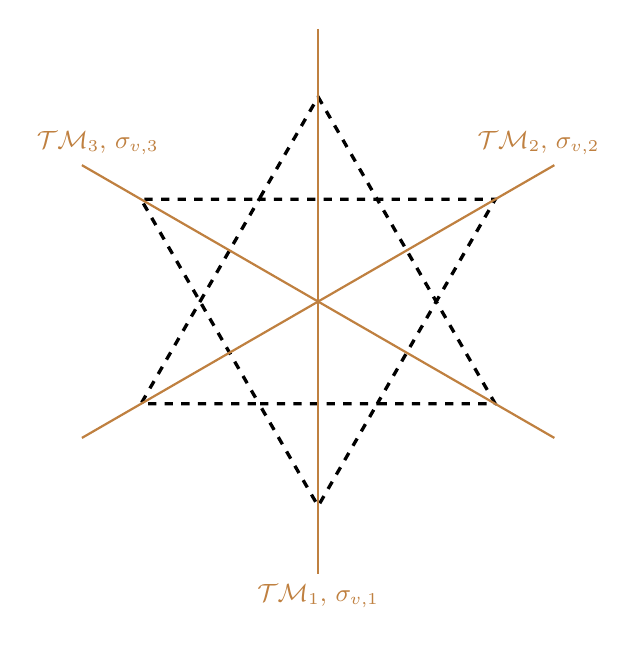
\begin{tikzpicture}[scale=1.5]
    
      % half-length of each spin arrow
      \def\spinhalf{0.3}
    
      % angles of the three sublattices
      \def\phiA{90}
      \def\phiB{210}
      \def\phiC{330}
    
      % useful constants
      \pgfmathsetmacro{\rt}{sqrt(3)}
      \pgfmathsetmacro{\rthalf}{sqrt(3)/2}
    
      % lattice
      \draw[very thick, dashed]
        (0,0) -- (0.5,\rthalf) -- (1.5,\rthalf) -- (2,0)
        -- (1.5,-\rthalf) -- (0.5,-\rthalf) -- (0,0)
        -- (-0.5,\rthalf) -- (0.5,\rthalf) -- (1,\rt)
        -- (1.5,\rthalf) -- (2.5,\rthalf) -- (2,0)
        -- (2.5,-\rthalf) -- (1.5,-\rthalf) -- (1,-\rt)
        -- (0.5,-\rthalf) -- (-0.5,-\rthalf) -- (0,0);

             \draw[thick, brown] (-1, {-2*sqrt(3)/3}) -- (3, {2*sqrt(3)/3}) node[above left,  xshift= 20pt, font=\small]{$\mathcal{TM}_2$, $\sigma_{v,2}$};
          \draw[thick, brown] (1,{4*sqrt(3)/3}) -- (1,{-4*sqrt(3)/3}) node[below, font=\small]{$\mathcal{TM}_1$, $\sigma_{v,1}$};
            \draw[thick, brown] (3, {-2*sqrt(3)/3}) -- (-1, {2*sqrt(3)/3}) node[above right, xshift= -20pt, font=\small]{$\mathcal{TM}_3$, $\sigma_{v,3}$};   

 
      \foreach \x/\y in {
        1/{-\rt},
        0/0,
        1/{\rt},
        2/0
      }{
        \centerspin[pastelblue]{(\x,\y)}{\phiA}
      }
    
      % sublattice B
      \foreach \x/\y in {
        0.5/{\rthalf},
        1.5/{-\rthalf},
        -0.5/{-\rthalf},
        2.5/{\rthalf}
      }{
        \centerspin[pastelred]{(\x,\y)}{\phiB}
      }
    
      % sublattice C
      \foreach \x/\y in {
        0.5/{-\rthalf},
        1.5/{\rthalf},
        -0.5/{\rthalf},
        2.5/{-\rthalf}
      }{
        \centerspin[pastelgreen]{(\x,\y)}{\phiC}
      }

    
    \end{tikzpicture}
    \caption{T1}
    \end{subfigure}
    \begin{subfigure}[c]{0.48\textwidth}
    \centering
        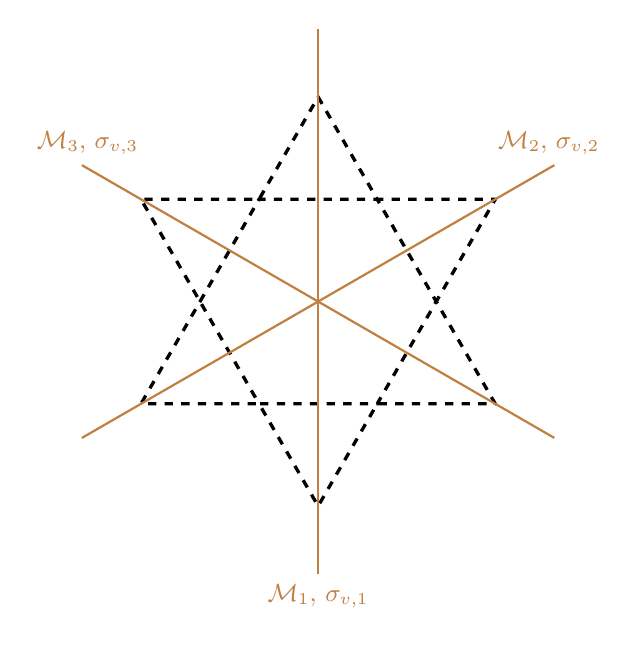
\begin{tikzpicture}[scale=1.5]
    
          % half-length of each spin arrow
          \def\spinhalf{0.3}
        
          % angles of the three sublattices
          \def\phiA{180}
          \def\phiB{300}
          \def\phiC{60}
        
          % useful constants
          \pgfmathsetmacro{\rt}{sqrt(3)}
          \pgfmathsetmacro{\rthalf}{sqrt(3)/2}
        
          % lattice
            \draw[very thick, dashed]
            (0,0) -- (0.5,\rthalf) -- (1.5,\rthalf) -- (2,0)
            -- (1.5,-\rthalf) -- (0.5,-\rthalf) -- (0,0)
            -- (-0.5,\rthalf) -- (0.5,\rthalf) -- (1,\rt)
            -- (1.5,\rthalf) -- (2.5,\rthalf) -- (2,0)
            -- (2.5,-\rthalf) -- (1.5,-\rthalf) -- (1,-\rt)
            -- (0.5,-\rthalf) -- (-0.5,-\rthalf) -- (0,0);
            
             \draw[thick, brown] (-1, {-2*sqrt(3)/3}) -- (3, {2*sqrt(3)/3}) node[above left,  xshift= 20pt, font=\small]{$\mathcal{M}_2$, $\sigma_{v,2}$};
          \draw[thick, brown] (1,{4*sqrt(3)/3}) -- (1,{-4*sqrt(3)/3}) node[below, font=\small]{$\mathcal{M}_1$, $\sigma_{v,1}$};
            \draw[thick, brown] (3, {-2*sqrt(3)/3}) -- (-1, {2*sqrt(3)/3}) node[above right,  xshift= -20pt, font=\small]{$\mathcal{M}_3$, $\sigma_{v,3}$};   

     
          % sublattice A
          \foreach \x/\y in {
            1/{-\rt},
            0/0,
            1/{\rt},
            2/0
          }{
            \centerspin[pastelblue]{(\x,\y)}{\phiA}
          }
        
          % sublattice B
          \foreach \x/\y in {
            0.5/{\rthalf},
            1.5/{-\rthalf},
            -0.5/{-\rthalf},
            2.5/{\rthalf}
          }{
            \centerspin[pastelred]{(\x,\y)}{\phiB}
          }
        
          % sublattice C
          \foreach \x/\y in {
            0.5/{-\rthalf},
            1.5/{\rthalf},
            -0.5/{\rthalf},
            2.5/{-\rthalf}
          }{
            \centerspin[pastelgreen]{(\x,\y)}{\phiC}
          }
        \end{tikzpicture}
    \caption{T2}
    \end{subfigure}
    \caption{\textbf{The magnetic order of the T1 and T2 phases of \ce{Mn3Pt}.} Illustrated are the conserved time-reversal mirror planes $\mathcal{TM}_i$ for the T1 phase and mirror planes $\mathcal{M}_i$ for T2 respectively. Additionally, the reflection symmetry planes $\sigma_{v,i}$, belonging to the $[C_{2\hat{s}}||\sigma_v]$ operation, are depicted on the corresponding kagome lattice.}
    \label{fig: magnetic texture Mn3Pt}
\end{figure}
    




The $\mathcal{TM}$ and $\mathcal{M}$ planes, as depicted in Fig.~\ref{fig: magnetic texture Mn3Pt}, impose constraints on the properties of the material according to Eqs.~\eqref{eq: symmetry_TM} and \eqref{eq: symmetry_M}, respectively. Note that for the $\mathcal{M}$ plane, the $[C_{2\hat{s}}||\sigma_v]$-symmetry is equivalent and therefore holds for SOC. 
The $\mathcal{TM}$ symmetry in the $yz$ plane is also preserved in the presence of SOC, which is shown in Section~\ref{section: Symmetries}. In combination to an additional $C_{3z}^s$ symmetry, shown below, there exist three $\mathcal{TM}$ planes imposing constraints also in the presence of SOC, due to $C_{3z}^s$ also preserved for SOC.  

Additionally, the symmetries introduced in Section~\ref{section: Symmetries}, namely the $\Theta_s[C_{2z}||E]$ and $[E||C_{2z}]$-symmetries, are expected to hold in \ce{Mn3Pt}. The former holds in the absence of SOC, while forcing the energy and in-plane spins to be even in $\mathbf{k}$ and out-of-plane spins and the Berry curvature to be odd. The latter holds in the nonbreathing limit, implying that the energy, spin and Berry curvature are even in momentum. \\

Because the T1 and T2 magnetic orders differ by a global spin rotation of $\pi/2$, equivalent results are expected in the absence of SOC up to the corresponding global spin rotation. With SOC, the phase difference acts differently on the Rashba Hamiltonian and therefore leads to different results.\\

The magnetic texture is invariant under a simultaneous real-space and spin-space rotation of $120^\circ$ around the $z$-axis, providing the $C_{3z}^s =[C_{3z}||C_{3z}]$ symmetry. This can be seen in Fig.~\ref{fig: magnetic texture Mn3Pt}.
The $C_{3z}^s$-symmetry is still preserved for Rashba SOC because its actions in spin- and real-space are equivalent. 
This symmetry further leads to a $C_{3z}$-symmetric behavior of the energy, spin, and Berry curvature given by 

\begin{align}
    E_n(C_{3z}\mathbf k)&=E_m(\mathbf k) \nonumber\\
    \mathbf s_n(C_{3z}\mathbf k)
  &=C_{3z}\mathbf s_m(\mathbf k) \nonumber\\
    \Omega_{xy}^{(n)}(C_{3z}\mathbf k)
  &=\Omega_{xy}^{(m)}(\mathbf k). 
    \label{eq: C_3z^s symm}
\end{align}
Here, the band indices may coincide, i.e., $n=m$. This symmetry forces the in-plane net magnetization of both phases of \ce{Mn3Pt} to vanish. Therefore, we expect an in-plane antiferromagnetic behavior with spin-split bands. \\
Furthermore, $[C_{2\hat{s}}||\sigma_v]$ requires the out-of-plane net magnetization $M_z$ to vanish for a coplanar magnetic texture. Because this symmetry breaks for the T1 phase in the case of SOC, this phase may acquire an out-of-plane magnetization in the presence of SOC. 

By contrast, this symmetry holds for SOC in the T2 phase, implying $M_z=0$. Hence, the T2 phase has a zero net magnetization ($M=0$), even in the presence of SOC. Because the in-plane magnetization vanishes for both phases, both altermagnets can be classified as S-type altermagnets, as introduced in Ref.~\cite{Cheong2025}. 

\subsection{Electronic structure of the T1 phase}
\label{subsubsection: T1 phase}
The band structures for the nonbreathing limit and for a breathing lattice are computed separately by diagonalizing the Hamiltonian in Eq.~\eqref{eq: bloch-Hamiltonian}. With the eigenstates of the Hamiltonian, the in-plane momentum space spin texture is obtained, given by Eq.~\eqref{eq: spin expectation}, which is evaluated on the contour of the Fermi surface. The Fermi surface is the set of momenta $\mathbf{k}$ satisfying $E_n(\mathbf{k})=\mu$, where $\mu$ is the chemical potential.
Figs.~\ref{fig:Mn3Pt1-nonbreathing} (a) and (b) show the computed band structures and the in-plane Fermi-surface spin textures for the nonbreathing limit, whereas Figs.~\ref{fig:Mn3Pt1-breathing} (a) and (b) show them for a breathing kagome lattice. 
The Berry curvature is finally computed by using the Fukui-Hatsugai-Suzuki method, explained in Section~\ref{section: Berrycurv}, where, for bands with degeneracies, the composite Berry curvature is computed. The selected band multiplets are indicated in the Berry curvature panels and are mostly treated consistently across the parameter sets. Thus, it may occur that a band multiplet is chosen, even if the bands in it are not degenerate. However, if the band multiplet is isolated, neither the value of its composite Chern number nor, more importantly, the symmetry constraints on its composite Berry curvature change.\\

In the nonbreathing limit, we expect the energy, the spin texture, and Berry curvature to be even in $\mathbf{k}$, which is confirmed in Fig.~\ref{fig:Mn3Pt1-nonbreathing}. 
The $\mathcal{TM}$ planes are visible with SOC, matching our expectations. 
\\
In the case without SOC, the $\Theta_s[C_{2z}||E]$-symmetry leads to an odd Berry curvature and, together with the evenness imposed by $[E||C_{2z}]$, forces the Berry curvature to vanish. Thus, the Chern number also vanishes. 
In the nonbreathing limit, as well as in the breathing lattice, a $C_{3z}^s$-symmetry can be observed, due to the magnetic texture being invariant under the action of the symmetry.

It can also be noted that the degeneracies at $M$ and $\Gamma$ are compatible with our expectations, stemming from the energy being even in $\mathbf{k}$ because then 
\begin{align}
    E_n(M) &= E_m(-M) = E_m(\mathbf{G}-M)
    \label{eq: degeneracy_even_for_M}\\
    E_n(\Gamma) &= E_m(-\Gamma) = E_m(\mathbf{G}-\Gamma).
    \label{eq: degeneracy_even_for_Gamma}
\end{align}
Here, the ability to fold back into the Brillouin zone by a reciprocal vector $\mathbf{G}$ is used. 
\begin{figure}[tbhp]
    \centering
    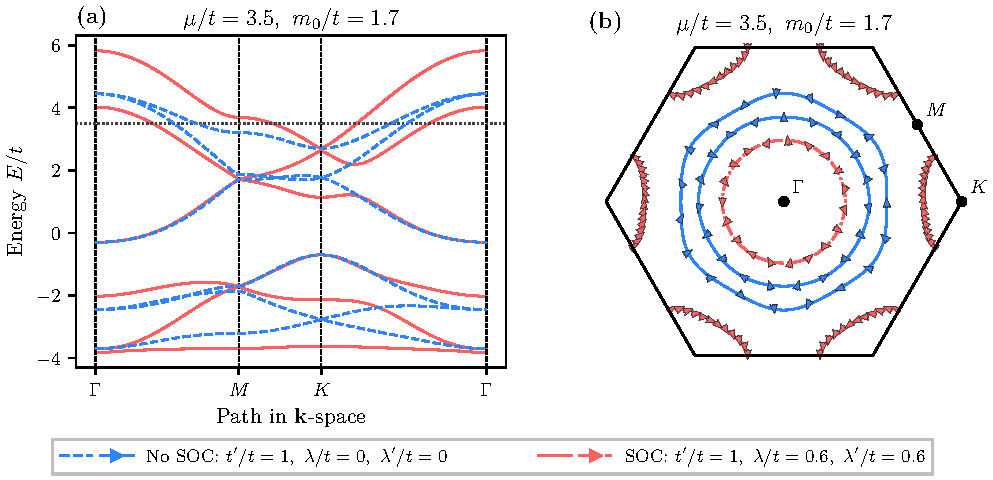
\includegraphics[
        width=\linewidth
    ]{Plots/Mn3Pt T1/Mn3Pt1 nonbreathing.pdf}
    \par\bigskip
    \begin{subfigure}[t]{0.46\textwidth}
        \centering
        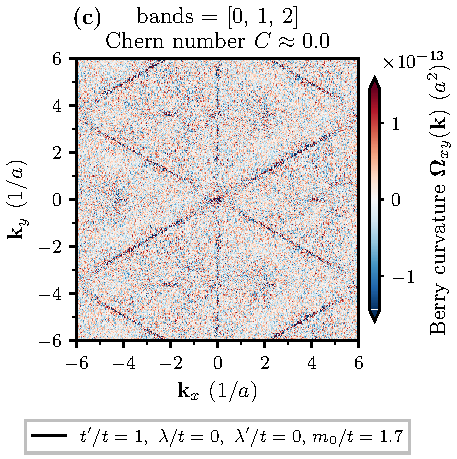
\includegraphics[
            width=\linewidth
        ]{Plots/Mn3Pt T1/Mn3Pt1 nonbreathing_berry_wo_soc.pdf}
        
    \end{subfigure}
    \hfill
    \begin{subfigure}[t]{0.48\textwidth}
        \centering
        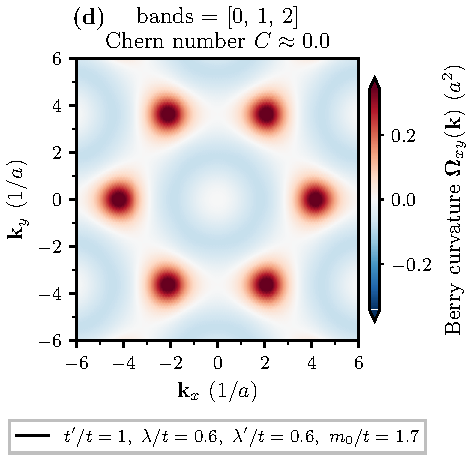
\includegraphics[
            width=\linewidth
        ]{Plots/Mn3Pt T1/Mn3Pt1 nonbreathing_berry_w_soc.pdf}
        
    \end{subfigure}
    \caption{\textbf{Tight-binding results for the T1 phase of \ce{Mn3Pt} in the nonbreathing limit, with the magnetic texture shown in Fig.~\ref{fig: magnetic texture Mn3Pt} (a), obtained using the Bloch Hamiltonian in Eq.~\eqref{eq: bloch-Hamiltonian}.} (a) Electronic band structure along the high-symmetry path $\Gamma$--$M$--$K$. (b) In-plane spin texture on the Fermi surface at the chemical potential $\mu$. (c,d) Berry curvature calculated without and with spin--orbit coupling (SOC), respectively, using the Fukui--Hatsugai--Suzuki method described in Eq.~\eqref{eq: berry curv comp}.}
    \label{fig:Mn3Pt1-nonbreathing}
\end{figure}
This argument does not work for $K$ because $K+\mathbf{G} = -K\neq K$. However, it can be argued by using $[C_{3z}||C_{3z}]$ and evenness in $\mathbf{k}$ that a degeneracy at $K$ is allowed given by 
\begin{align}
    E_n(K) = E_m(-K) = E_\ell(-C_{3z}K) = E_\ell(K'+\mathbf{G}) = E_\ell(K)
    \label{eq: degeneracy_C3z_even_for_K}
\end{align}
with $K' = -K $.
Note that we did not show that $n \neq \ell$ or $n\neq m$ and therefore the symmetry arguments do not prove that this degeneracy occurs. They only provide an explanation for degeneracies that may occur at the given $\mathbf{k}$-points. \\


For the breathing kagome lattice, we expect the $[E||C_{2\hat{z}}]$-symmetry to be broken and therefore the energy, spin and Berry curvature not to be generally even in $\mathbf{k}$, as confirmed in Fig.~\ref{fig:Mn3Pt1-breathing}. However, in the absence of SOC, $\Theta_s[C_{2z}||E]$ still forces the in-plane spins and energies to be even and the Berry curvature to be odd in $\mathbf{k}$, as observed in Fig.~\ref{fig:Mn3Pt1-breathing}. Therefore, even when $[E||C_{2\hat{z}}]$ is broken, the energy and in-plane spins remain even in the absence of SOC. Additionally, the out-of-plane spin component is expected to be odd in $\mathbf{k}$.\\

We also observe a $C_{3z}^s$-symmetry as expected.

% Lastly, we note that the $\mathcal{TM}$-plane is visible for all chosen cases, however, by using numerical calculations, we show, with the use of OpenAI's 'ChatGPT' for helping with the creation of the code, that the $\mathcal{TM}$-symmetry is actually slightly broken for SOC, as expected. \\
% For this, we use $U_{TM} \mathfrak
% {H}(\mathbf{k})^*U_{TM} = \mathfrak
% {H}(-\mathcal{M}\mathbf{k})$ with $U_{{TM}} = P \otimes U_{TM}^{\text{spin}} = P \otimes U_{M}^\text{spin}i\sigma_y\mathcal{K}$, where we use the spatial mirror $P$, assigning the sublattices onto the according position, and the spinful mirror operator $U_\mathcal{M}^\text{spin}$, rotating the spins perpendicular to the mirror plane because of the pseudovectorial characteristics of spins. \\

\begin{figure}[tbhp]
    \centering
    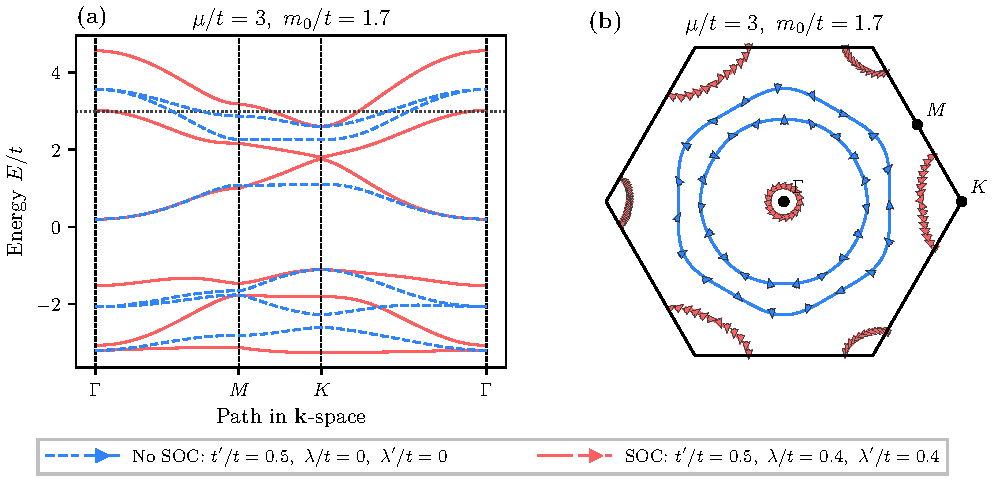
\includegraphics[
        width=\linewidth
    ]{Plots/Mn3Pt T1/Mn3Pt1 breathing.pdf}
    \par\bigskip
    \begin{subfigure}[t]{0.48\textwidth}
        \centering
        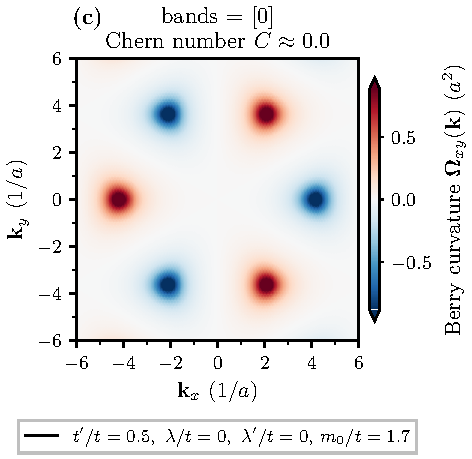
\includegraphics[
            width=\linewidth
        ]{Plots/Mn3Pt T1/Mn3Pt1 breathing_berry_wo_soc.pdf}
        
    \end{subfigure}
    \hfill
    \begin{subfigure}[t]{0.48\textwidth}
        \centering
        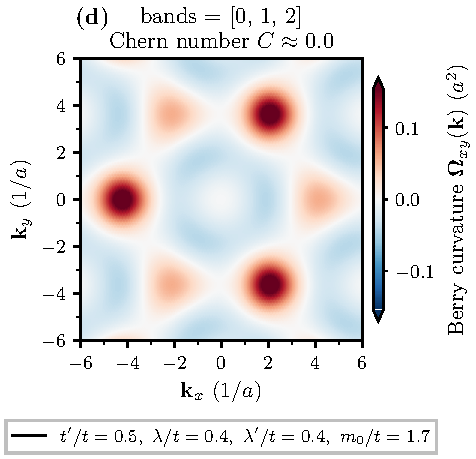
\includegraphics[
            width=\linewidth
        ]{Plots/Mn3Pt T1/Mn3Pt1 breathing_berry_w_soc.pdf}
        
    \end{subfigure}
    \caption{\textbf{Tight-binding results for the T1 phase of \ce{Mn3Pt} in a breathing lattice, with the magnetic texture shown in Fig.~\ref{fig: magnetic texture Mn3Pt} (a), obtained using the Bloch Hamiltonian in Eq.~\eqref{eq: bloch-Hamiltonian}.} (a) Electronic band structure along the high-symmetry path $\Gamma$--$M$--$K$. (b) In-plane spin texture on the Fermi surface at the chemical potential $\mu$. (c,d) Berry curvature calculated without and with spin--orbit coupling (SOC), respectively, using the Fukui--Hatsugai--Suzuki method described in Eq.~\eqref{eq: berry curv comp}.}
    \label{fig:Mn3Pt1-breathing}
\end{figure}

Lastly, we observe $[C_{2\hat{s}}||\sigma_v]$ in the absence of SOC and the $\mathcal{TM}$ planes, depicted in Fig.~\ref{fig: magnetic texture Mn3Pt} (a). The $\mathcal{TM}$-typical behavior is given by Eq.~\eqref{eq: symmetry_TM} and is also observed in a numerical calculation in the presence of SOC. Therefore, we observe our data to be compatible with a $\mathcal{TM}$ symmetry as expected due to a conserved $\mathcal{TM}$ and $C_{3z}^s$ symmetry in the presence of SOC.  
\FloatBarrier
\subsection{Electronic structure of the T2 phase}
Similarly to the T1 phase, we compute the band structure, Fermi-surface spin textures and Berry curvature as depicted in Figs.~\ref{fig:Mn3Pt2-nonbreathing} and \ref{fig:Mn3Pt2-breathing}.
A similar behavior in comparison to the T1 phase is observed. The principal difference is that the T2 phase has $\mathcal{M}$ planes rather than the $\mathcal{TM}$ planes of T1 and an additional global phase shift, as shown in Fig.~\ref{fig: magnetic texture Mn3Pt} (b). 
\\
Similar symmetry arguments for the occurrence of degeneracies, as given in Eqs.~\eqref{eq: degeneracy_C3z_even_for_K},~\eqref{eq: degeneracy_even_for_Gamma} and \eqref{eq: degeneracy_even_for_M}, can be applied to the T2 phase, and therefore degeneracies at $K$, $\Gamma$ and $M$ are permitted if the energy is even in $\mathbf{k}$.

\begin{figure}[tbhp]
    \centering
    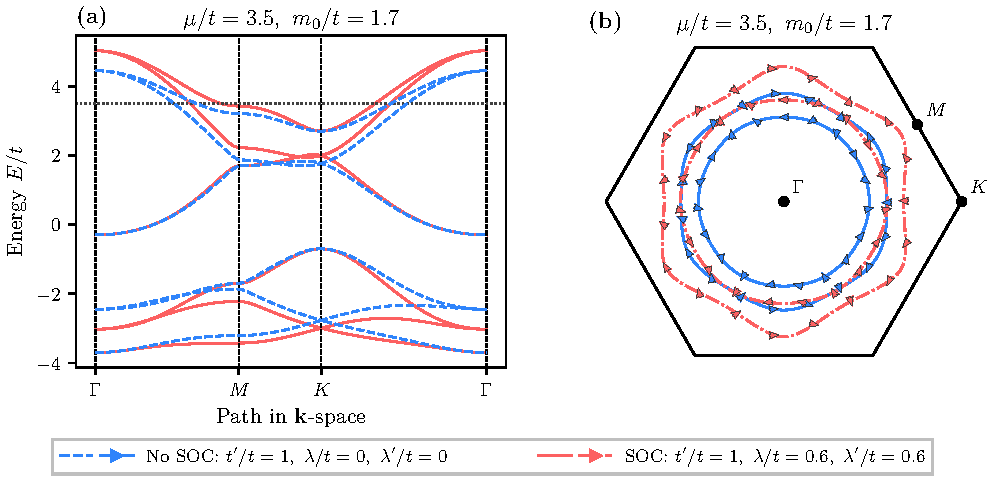
\includegraphics[
        width=\linewidth
    ]{Plots/Mn3Pt T2/Mn3Pt2 nonbreathing.pdf}
    \par\bigskip
    \begin{subfigure}[t]{0.48\textwidth}
        \centering
        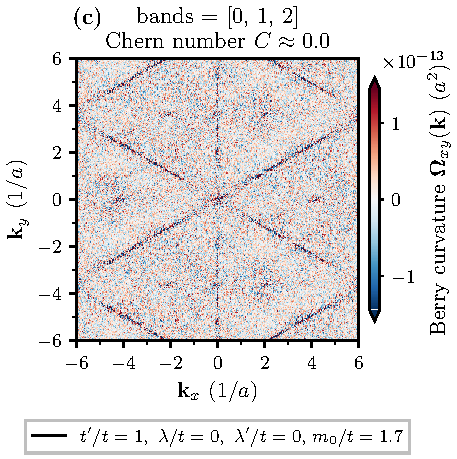
\includegraphics[
            width=\linewidth
        ]{Plots/Mn3Pt T2/Mn3Pt2 nonbreathing_berry_wo_soc.pdf}
        
    \end{subfigure}
    \hfill
    \begin{subfigure}[t]{0.48\textwidth}
        \centering
        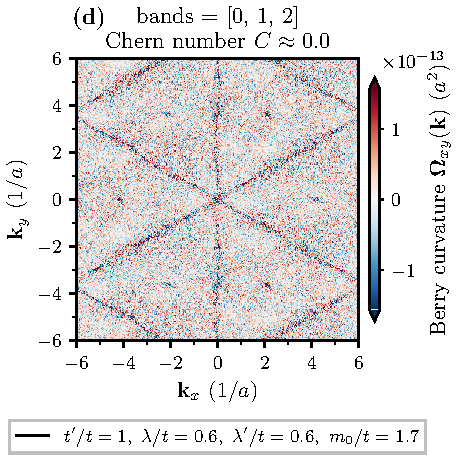
\includegraphics[
            width=\linewidth
        ]{Plots/Mn3Pt T2/Mn3Pt2 nonbreathing_berry_w_soc.pdf}
        
    \end{subfigure}
    \caption{\textbf{Tight-binding results for the T2 phase of \ce{Mn3Pt} in the nonbreathing limit, with the magnetic texture shown in Fig.~\ref{fig: magnetic texture Mn3Pt} (b), obtained using the Bloch Hamiltonian in Eq.~\eqref{eq: bloch-Hamiltonian}.} (a) Electronic band structure along the high-symmetry path $\Gamma$--$M$--$K$. (b) In-plane spin texture on the Fermi surface at the chemical potential $\mu$. (c,d) Berry curvature calculated without and with spin--orbit coupling (SOC), respectively, using the Fukui--Hatsugai--Suzuki method described in Eq.~\eqref{eq: berry curv comp}.}
    \label{fig:Mn3Pt2-nonbreathing}
\end{figure}
The two phases give equivalent results in the absence of SOC, as seen by comparing Figs.~\ref{fig:Mn3Pt1-nonbreathing} and \ref{fig:Mn3Pt2-nonbreathing} or Figs.~\ref{fig:Mn3Pt1-breathing} and \ref{fig:Mn3Pt2-breathing} due to the global spin rotation of $\pi/2$, shown in Fig.~\ref{fig: magnetic texture Mn3Pt}. Therefore, the spin texture is expected to be rotated by an additional global phase of $\pi/2$ for the T2 phase in the absence of SOC.
The Berry curvature vanishes in the mirror-invariant plane $\mathcal{M}$, as observed in Fig.~\ref{fig:Mn3Pt2-breathing}, and the behavior according to Eq.~\eqref{eq: symmetry_M} is observed for energy, in-plane spin and Berry curvature in Figs.~\ref{fig:Mn3Pt2-nonbreathing} and \ref{fig:Mn3Pt2-breathing}. Thus, the mirror plane is observed in the electronic-structure properties. The vanishing of the Berry curvature on the mirror-invariant plane stems from it being odd under the mirror plane. In the Fermi-surface spin textures, the spin on the mirror plane is expected to be perpendicular to the mirror plane. \\
We again observe the $C_{3z}$ behavior and, without SOC, even energies and in-plane spins but an odd Berry curvature, where the former is imposed by $C_{3z}^s$ and the latter by $\Theta_s[C_{2z}||E]$.
Thus, the Berry curvature vanishes in the absence of SOC in the nonbreathing limit. We also observe that the Berry curvature vanishes in the presence of SOC in the nonbreathing limit. Although this result would be consistent with an additional $\mathcal{TM}$ symmetry in the $xz$-plane, which could occur only
in the nonbreathing limit, such a symmetry has not been established for the full Hamiltonian. Therefore, a future study would have to show this. Hence, we treat this as a numerical observation. Nevertheless, independently of the additional symmetry plane, the Chern number is forced to zero due to the conserved $\mathcal{M}$ symmetry.
\begin{figure}[tbhp]
    \centering
    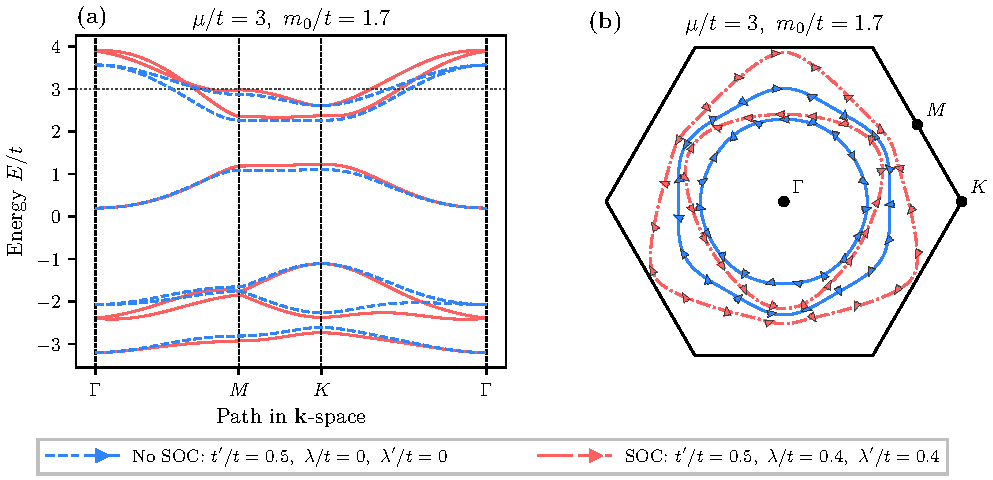
\includegraphics[
        width=\linewidth
    ]{Plots/Mn3Pt T2/Mn3Pt2 breathing.pdf}
    \par\bigskip
    \begin{subfigure}[t]{0.48\textwidth}
        \centering
        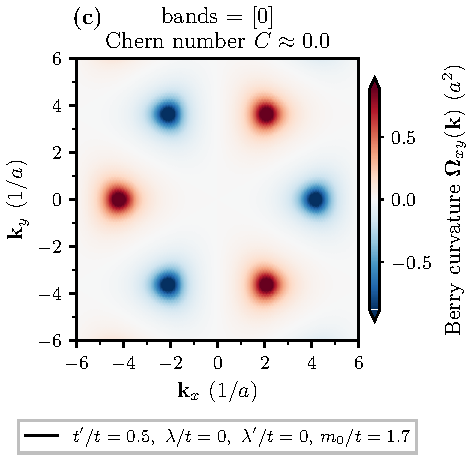
\includegraphics[
            width=\linewidth
        ]{Plots/Mn3Pt T2/Mn3Pt2 breathing_berry_wo_soc.pdf}
        
    \end{subfigure}
    \hfill
    \begin{subfigure}[t]{0.48\textwidth}
        \centering
        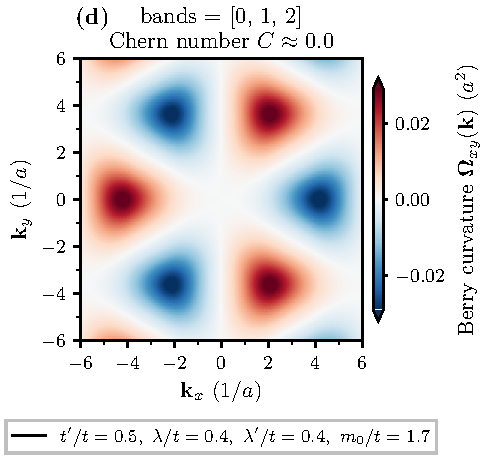
\includegraphics[
            width=\linewidth
        ]{Plots/Mn3Pt T2/Mn3Pt2 breathing_berry_w_soc.pdf}
        
    \end{subfigure}
    \caption{\textbf{Tight-binding results for the T2 phase of \ce{Mn3Pt} in a breathing lattice, with the magnetic texture shown in Fig.~\ref{fig: magnetic texture Mn3Pt} (b), obtained using the Bloch Hamiltonian in Eq.~\eqref{eq: bloch-Hamiltonian}.} (a) Electronic band structure along the high-symmetry path $\Gamma$--$M$--$K$. (b) In-plane spin texture on the Fermi surface at the chemical potential $\mu$. (c,d) Berry curvature calculated without and with spin--orbit coupling (SOC), respectively, using the Fukui--Hatsugai--Suzuki method described in Eq.~\eqref{eq: berry curv comp}.}
    \label{fig:Mn3Pt2-breathing}
\end{figure}

The alternating form of the Berry curvature for a breathing lattice comes from the combination of $C_{3z}^s$ and the mirror plane $\mathcal{M}$. An odd behavior of the Berry curvature is not expected in the presence of SOC, and can be checked numerically by calculating
\begin{align}
\frac{\max_{\mathbf{k}}\left|\Omega_{xy}^{(n)}(\mathbf{k})+\Omega_{xy}^{(n)}(-\mathbf{k})\right|}{\max_{\mathbf{k}}\left|\Omega_{xy}^{(n)}(\mathbf{k})\right|}\approx 0.02, \nonumber
\end{align}
which yields numerical nonzero values and therefore no odd behavior of the Berry curvature.
In the absence of SOC for the breathing case, the energy and in-plane spins are as expected even, whereas the Berry curvature is odd.
\newpage
\section{M-type altermagnetism in \ce{Mn3Ge} and \ce{Mn3Sn}}
In this section, the model and symmetries formulated in Chapter~\ref{chapter:Theory} are applied to the magnetic texture of the M-type altermagnets \ce{Mn3Ge} and \ce{Mn3Sn}. 
Further, the expectations are compared with the computed results of the band structure, in-plane Fermi-surface spin texture and the out-of-plane component of Berry curvature.

\subsection{Magnetic structures and symmetries of \ce{Mn3Ge} and \ce{Mn3Sn}}

Similarly to \ce{Mn3Pt}, a kagome lattice consisting of manganese atoms in \ce{Mn3Ge} and \ce{Mn3Sn} is obtained by projecting the atoms onto the $(0001)$-plane in the hexagonal structure $D0_{19}$, as stated, for example, in Ref.~\cite{10.1063/1.5064697}. Here, the localized magnetic moments reside predominantly on the manganese atoms due to nearly filled orbitals of the $\ce{Ge}$ and $\ce{Sn}$ atoms, thus weak magnetic moments. \\
The magnetic moments form a triangular $120^\circ$ order and therefore the structures depicted in Figs.~\ref{fig: magnetic texture Mn3Ge and Sn}~(a) and (b) are consistent with the magnetic point groups $m'mm'$ and $mm'm'$, respectively.\\
For \ce{Mn3Ge}, the phases of the magnetic texture in Fig.~\ref{fig: magnetic texture Mn3Ge and Sn} are $\varphi_{3,A} = \pi/2$, $\varphi_{3,B} = 11\pi/6$ and $\varphi_{3,C}= 7\pi/6$. The magnetic texture of \ce{Mn3Sn} is obtained by adding a global spin rotation of $\pi/2$ to the magnetic moments.\\

In the magnetic texture, the symmetry $[C_{3z}||C_{3z}^{-1}]$ is found, which combines a $120^\circ$ spin-space rotation and a $-120^\circ$ spatial rotation. This symmetry stems from the magnetic order, depicted in Fig.~\ref{fig: magnetic texture Mn3Ge and Sn}, which can be verified using the relations
\begin{align}
    A\to B & \qquad  \varphi_B = \varphi_A -\frac{2\pi}{3} \nonumber \\
    B\to C & \qquad \varphi_C = \varphi_B -\frac{2\pi}{3} \nonumber  \\
    C\to A & \qquad \varphi_A = \varphi_C -\frac{2\pi}{3}.
\end{align}
Therefore, we expect the relations given by

\begin{align}
    E_m(C_{3z}\mathbf k)&=E_n(\mathbf k) \nonumber\\
    \mathbf s_m(C_{3z}\mathbf k)
  &=C_{3z}^{-1}\mathbf s_n(\mathbf k) \nonumber\\
    \Omega_{xy}^{(m)}(C_{3z}\mathbf k)
  &=\Omega_{xy}^{(n)}(\mathbf k),
    \label{eq: C_3z^-1 symm}
\end{align}
analogous to Eq.~\eqref{eq: C_3z^s symm}, in the absence of SOC. The symmetry breaks in the presence of SOC, due to inequivalent transformations for spin- and real-space.
The symmetry also fixes the in-plane net magnetization to zero, analogously to $C_{3z}^s$ for \ce{Mn3Pt}, in the absence of SOC.

The $\mathcal{M}$ and $\mathcal{TM}$ planes depicted in Fig.~\ref{fig: magnetic texture Mn3Ge and Sn} impose the constraints in Eq.~\eqref{eq: symmetry_M} and \eqref{eq: symmetry_TM}.
The conservation of the $\mathcal{M}$ and $\mathcal{TM}$ symmetries in the presence of SOC is shown in Section~\ref{section: Symmetries}. 
Additionally, we argue that the mirror plane $\mathcal{M}$, which is in this case equal to $[C_{2\hat{s}}||\sigma_v]$ because the spin is perpendicular to the mirror plane, is preserved in the presence of SOC due to $[C_{2\hat{s}}||\sigma_v]$ transforming spin-space and real-space equivalently.
Thus, the $\mathcal{M}$ and $\mathcal{TM}$ planes are expected to be visible in the presence of SOC.

In contrast, the $[C_{2\hat{\mathbf{s}}}||\sigma_v]$ operator, whose plane is depicted in Fig.~\ref{fig: magnetic texture Mn3Ge and Sn}, is broken by SOC in \ce{Mn3Ge} because the spin at the mirror-invariant site lies within the mirror plane, therefore, the spin-space and spatial transformations are inequivalent.   \\


%NEEEL TEMPERATURE https://www.sciencedirect.com/science/article/abs/pii/S0304885322009039 365K - 400K!!!

\begin{figure}[tbhp]
    \centering
    % First Subfigure
    \begin{subfigure}[c]{0.48\textwidth}
        \centering
        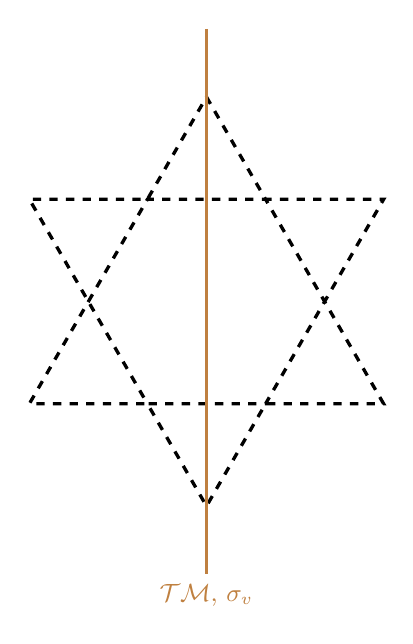
\begin{tikzpicture}[scale=1.5]
        
          % half-length of each spin arrow
          \def\spinhalf{0.3}
        
          % angles of the three sublattices
          \def\phiA{90}
          \def\phiB{330}
          \def\phiC{210}
        
          % useful constants
          \pgfmathsetmacro{\rt}{sqrt(3)}
          \pgfmathsetmacro{\rthalf}{sqrt(3)/2}
        
          % lattice
          \draw[very thick, dashed]
            (0,0) -- (0.5,\rthalf) -- (1.5,\rthalf) -- (2,0)
            -- (1.5,-\rthalf) -- (0.5,-\rthalf) -- (0,0)
            -- (-0.5,\rthalf) -- (0.5,\rthalf) -- (1,\rt)
            -- (1.5,\rthalf) -- (2.5,\rthalf) -- (2,0)
            -- (2.5,-\rthalf) -- (1.5,-\rthalf) -- (1,-\rt)
            -- (0.5,-\rthalf) -- (-0.5,-\rthalf) -- (0,0);
            
          \draw[thick, brown] (1,{4*sqrt(3)/3}) -- (1,{-4*sqrt(3)/3}) node[below, font=\small]{$\mathcal{TM}$, $\sigma_v$};
          % sublattice A
          \foreach \x/\y in {
            1/{-\rt},
            0/0,
            1/{\rt},
            2/0
          }{
            \centerspin[pastelblue]{(\x,\y)}{\phiA}
          }
        
          % sublattice B
          \foreach \x/\y in {
            0.5/{\rthalf},
            1.5/{-\rthalf},
            -0.5/{-\rthalf},
            2.5/{\rthalf}
          }{
            \centerspin[pastelred]{(\x,\y)}{\phiB}
          }
        
          % sublattice C
          \foreach \x/\y in {
            0.5/{-\rthalf},
            1.5/{\rthalf},
            -0.5/{\rthalf},
            2.5/{-\rthalf}
          }{
            \centerspin[pastelgreen]{(\x,\y)}{\phiC}
          }

        \end{tikzpicture}
    \caption{\ce{Mn3Ge}}
    \label{fig: magnetic texture Mn3Ge}
    \end{subfigure}
    \begin{subfigure}[c]{0.48\textwidth}
    \centering
    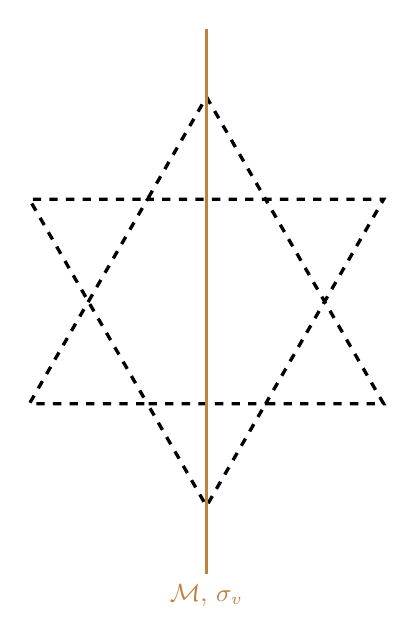
\begin{tikzpicture}[scale=1.5]
    
      % half-length of each spin arrow
      \def\spinhalf{0.3}
    
      % angles of the three sublattices
      \def\phiA{0}
      \def\phiB{240}
      \def\phiC{120}
    
      % useful constants
      \pgfmathsetmacro{\rt}{sqrt(3)}
      \pgfmathsetmacro{\rthalf}{sqrt(3)/2}
    
      % lattice
      \draw[very thick, dashed]
        (0,0) -- (0.5,\rthalf) -- (1.5,\rthalf) -- (2,0)
        -- (1.5,-\rthalf) -- (0.5,-\rthalf) -- (0,0)
        -- (-0.5,\rthalf) -- (0.5,\rthalf) -- (1,\rt)
        -- (1.5,\rthalf) -- (2.5,\rthalf) -- (2,0)
        -- (2.5,-\rthalf) -- (1.5,-\rthalf) -- (1,-\rt)
        -- (0.5,-\rthalf) -- (-0.5,-\rthalf) -- (0,0);
          \draw[thick, brown] (1,{4*sqrt(3)/3}) -- (1,{-4*sqrt(3)/3}) node[below, font=\small]{$\mathcal{M}$, $\sigma_v$};
      % sublattice A
      \foreach \x/\y in {
        1/{-\rt},
        0/0,
        1/{\rt},
        2/0
      }{
        \centerspin[pastelblue]{(\x,\y)}{\phiA}
      }
    
      % sublattice B
      \foreach \x/\y in {
        0.5/{\rthalf},
        1.5/{-\rthalf},
        -0.5/{-\rthalf},
        2.5/{\rthalf}
      }{
        \centerspin[pastelred]{(\x,\y)}{\phiB}
      }
    
      % sublattice C
      \foreach \x/\y in {
        0.5/{-\rthalf},
        1.5/{\rthalf},
        -0.5/{\rthalf},
        2.5/{-\rthalf}
      }{
        \centerspin[pastelgreen]{(\x,\y)}{\phiC}
      }

    
    \end{tikzpicture}
    \caption{\ce{Mn3Sn}}
    \label{fig: magnetic texture Mn3Sn}
    \end{subfigure}
    \caption{The magnetic order of (a) \ce{Mn3Ge} and (b) \ce{Mn3Sn}, as defined in Ref. \cite{Quelle1}, with the illustrated time-reversal mirror plane $\mathcal{TM}$ or mirror plane $\mathcal{M}$, respectively, and the reflection symmetry $\sigma_v$, belonging to $[C_{2\hat{s}}||\sigma_v]$, depicted on the corresponding kagome lattice. The magnetic order of \ce{Mn3Ge} has a time-reversal mirror plane, whereas that of \ce{Mn3Sn} has a mirror plane.}
    \label{fig: magnetic texture Mn3Ge and Sn}
\end{figure}

By analogy with \ce{Mn3Pt}, the symmetries $\Theta_s [C_{2z}||E]$ and $[E||C_{2z}]$ are expected, where the former holds in the absence of SOC and the latter in the nonbreathing limit. 
Also, the two textures are predicted to behave identically in the absence of SOC with respect to the global spin rotation of $\pi/2$.\\
These symmetries constrain the direction of an allowed magnetization. When $[C_{3z}||C_{3z}^{-1}]$ is broken by adding SOC, a net magnetization is permitted in \ce{Mn3Ge} within the $\mathcal{TM}$ plane, i.e., along the $y$-axis, and in \ce{Mn3Sn} perpendicular to the $\mathcal{M}$ plane, i.e., along the $x$-axis.  



\subsection{Electronic structure of \ce{Mn3Ge}}
The computed band structure, in-plane Fermi-surface spin texture and Berry curvature are shown in Fig.~\ref{fig:Mn3Ge-nonbreathing} for the nonbreathing limit and in Fig.~\ref{fig:Mn3Ge-breathing} for a breathing kagome lattice.
\begin{figure}[tbhp]
    \centering
    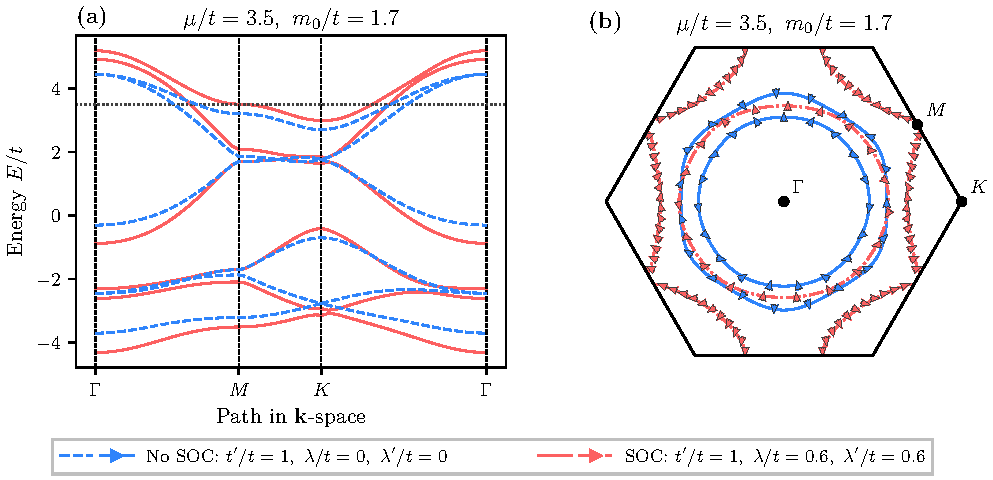
\includegraphics[
        width=\linewidth
    ]{Plots/Mn3Ge/Mn3Ge nonbreathing.pdf}
    \par\bigskip
    \begin{subfigure}[t]{0.46\textwidth}
        \centering
        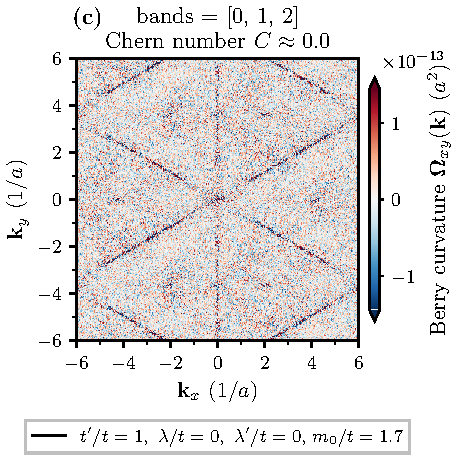
\includegraphics[
            width=\linewidth
        ]{Plots/Mn3Ge/Mn3Ge nonbreathing_berry_wo_soc.pdf}
        
    \end{subfigure}
    \hfill
    \begin{subfigure}[t]{0.48\textwidth}
        \centering
        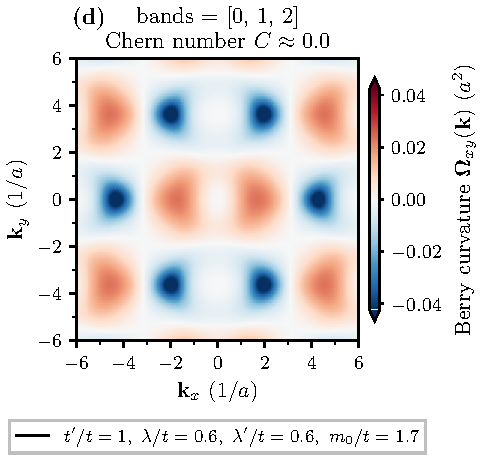
\includegraphics[
            width=\linewidth
        ]{Plots/Mn3Ge/Mn3Ge nonbreathing_berry_w_soc.pdf}
        
    \end{subfigure}
    \caption{\textbf{Tight-binding results for \ce{Mn3Ge} in the nonbreathing limit, with the magnetic texture shown in Fig.~\ref{fig: magnetic texture Mn3Ge and Sn}~(a), obtained using the Bloch Hamiltonian in Eq.~\eqref{eq: bloch-Hamiltonian}.} (a) Electronic band structure along the high-symmetry path $\Gamma$--$M$--$K$. (b) In-plane spin texture on the Fermi surface at the chemical potential $\mu$. (c,d) Berry curvature calculated without and with spin--orbit coupling (SOC), respectively, using the Fukui--Hatsugai--Suzuki method described in Eq.~\eqref{eq: berry curv comp}.}
\label{fig:Mn3Ge-nonbreathing}
\end{figure}
For the nonbreathing limit, the Berry curvature, energies, and spins are
even in $\mathbf{k}$, as imposed by $[E||C_{2z}]$, which also holds in the presence of SOC.\\
This operation and the $\Theta_s [C_{2z}||E]$ operator in the nonbreathing limit in the absence of SOC lead to a vanishing Berry curvature as seen in Fig.~\ref{fig:Mn3Ge-nonbreathing} (c), as also confirmed for \ce{Mn3Pt}. The imposed properties of $[C_{3z}||C_{3z}^{-1}]$, given by Eq.~\eqref{eq: C_3z^-1 symm}, are observed in the absence of SOC in Figs.~\ref{fig:Mn3Ge-nonbreathing} and \ref{fig:Mn3Ge-breathing}, therefore confirming the prediction. In the presence of SOC, $[C_{3z}||C_{3z}^{-1}]$ breaks. Thus, in the presence of SOC, the evenness, imposed by $[E||C_{2z}]$, is expected, as observed in Fig.~\ref{fig:Mn3Ge-nonbreathing}. \\
The properties imposed by $[C_{2\hat{s}}||\sigma_v]$ can also be observed in the absence of SOC. We are also able to observe properties imposed by the $\mathcal{TM}$ plane, according to Eq.~\eqref{eq: symmetry_TM}, in the case of SOC. Therefore, matching with our previously established expectations. \\

% The obtained results show a conservation of the $\mathcal{TM}$ plane for SOC of different orders using Eq.~\eqref{eq: TM symmetry prove eq}. \\
% It might be expected that this breakage is small enough for numerical errors to overtake. 
% Therefore, we are not able to confirm our theory for this case. !!!!!!!!!!!!!!!!!!!
% In Ref. \cite{MnPtSOC} it was confirmed, that the magnetic texture with SOC can be seen to get an out-of plane virtual texture and therefore breaking the $\mathcal{TM}$ plane. The angle of the virtual magnetic texture experiences a change of $\SI{0.15}{\degree}$, which confirms the seemingly holding $\mathcal{TM}$ plane. 
% !!!
\begin{figure}[tbhp]
    \centering
    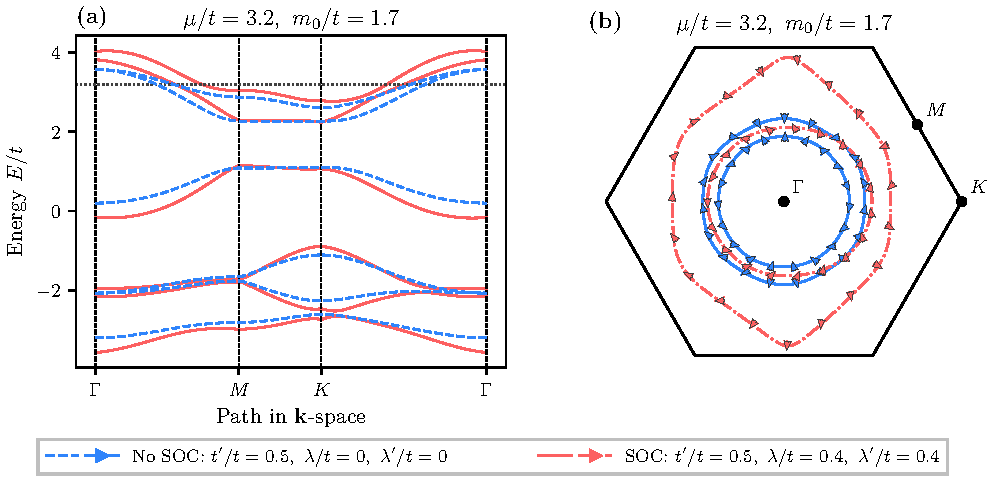
\includegraphics[
        width=\linewidth
    ]{Plots/Mn3Ge/Mn3Ge breathing.pdf}
    \par\bigskip
    \begin{subfigure}[t]{0.48\textwidth}
        \centering
        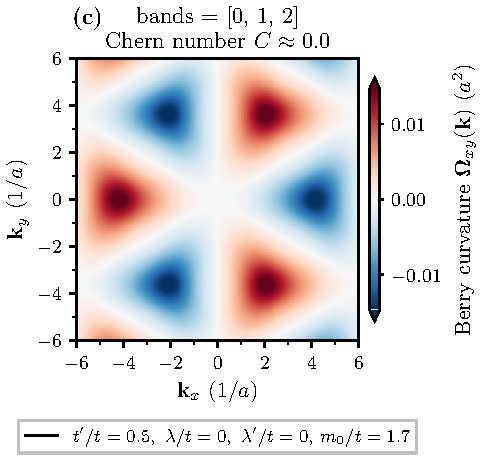
\includegraphics[
            width=\linewidth
        ]{Plots/Mn3Ge/Mn3Ge breathing_berry_wo_soc.pdf}
        
    \end{subfigure}
    \hfill
    \begin{subfigure}[t]{0.48\textwidth}
        \centering
        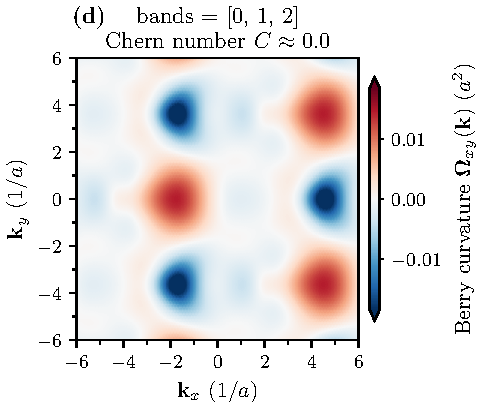
\includegraphics[
            width=\linewidth
        ]{Plots/Mn3Ge/Mn3Ge breathing_berry_w_soc.pdf}
        
    \end{subfigure}
    \caption{\textbf{Tight-binding results for \ce{Mn3Ge} in the breathing lattice, with the magnetic texture shown in Fig.~\ref{fig: magnetic texture Mn3Ge and Sn}~(a), obtained using the Bloch Hamiltonian in Eq.~\eqref{eq: bloch-Hamiltonian}.} (a) Electronic band structure along the high-symmetry path $\Gamma$--$M$--$K$. (b) In-plane spin texture on the Fermi surface at the chemical potential $\mu$. (c,d) Berry curvature calculated without and with spin--orbit coupling (SOC), respectively, using the Fukui--Hatsugai--Suzuki method described in Eq.~\eqref{eq: berry curv comp}.}
    \label{fig:Mn3Ge-breathing}
\end{figure}
Breaking the nonbreathing limit by introducing unequal hopping parameters breaks
the symmetry $[E||C_{2z}]$ that otherwise imposes evenness, thereby allowing a nonzero Berry curvature in the absence of SOC, which was earlier prohibited by $\Theta_s[C_{2z}||E]$ and $[E||C_{2z}]$. Therefore, we are able to observe the odd behavior of the Berry curvature, imposed by $\Theta_s [C_{2z}||E]$, forcing the total Chern number of an isolated composite subspace to vanish, as seen in Fig.~\ref{fig:Mn3Ge-breathing}~(c). \\
The energy and spins are even in the absence of SOC, whereas the Berry curvature is odd, due to $\Theta_s[C_{2z}||E]$. These constraints, together with $[C_{3z}||C_{3z}^{-1}]$ and the $\mathcal{TM}$ plane, lead to the observed behavior in Fig.~\ref{fig:Mn3Ge-breathing}.\\
In the presence of SOC in the breathing lattice, $\Theta_s [C_{2z}||E]$, $[C_{2\hat{s}}||\sigma_v]$ and $[C_{3z}||C_{3z}^{-1}]$ are broken. The only observable properties are the imposed constraints of the $\mathcal{TM}$ symmetry, given by Eq.~\eqref{eq: symmetry_TM}. Thus, the resulting numerical data are compatible with the expected $\mathcal{TM}$ symmetry, conserved in the presence of SOC.\\

In \ce{Mn3Ge}, a net magnetization along the $\mathcal{TM}$ plane, or along $y$, can be formed in the presence of SOC. This is because $[C_{3z}||C_{3z}^{-1}]$ is broken, which allows an in-plane net magnetization, and the $\mathcal{TM}$ plane itself forces the perpendicular component, or, the net magnetization along $x$, to vanish. Thus, a net magnetization is allowed in the $y$-direction. \\
The effects of the resulting net magnetization can be observed in the Fermi-surface spin texture in Figs.~\ref{fig:Mn3Ge-nonbreathing} and \ref{fig:Mn3Ge-breathing} in the case of SOC. We next discuss the origin of the deformation of the Fermi surface. The symmetry plane constrains spins along $k_y=0$ to align along $y$ or with the net magnetization. Using the Rashba term, according to Eq.~\eqref{eq: Rashba_Hamiltonian_standard} and evaluating its expectation value with the eigenstates, we obtain
\begin{align}
    \Delta E_{\text{R},n}=\alpha_{\mathrm R}k_x\langle\sigma_y\rangle_n.
\end{align}
Therefore, opposite $y$-directed spin expectation values experience an energy shift of opposite sign, producing a deformation along $k_x$, as observed in Figs.~\ref{fig:Mn3Ge-nonbreathing} and \ref{fig:Mn3Ge-breathing}.
Thus, Rashba coupling produces a deformation in the Fermi surface perpendicular to the magnetization.


Figs.~\ref{fig:Mn3Ge-nonbreathing} and \ref{fig:Mn3Ge-breathing} show that the bands are spin-split also in the absence of SOC, classifying \ce{Mn3Ge} as a strong altermagnet. The spin-splitting arises because the compensated texture breaks $\mathcal{PT}$ symmetry and other symmetries that would enforce band degeneracies.


Hence, \ce{Mn3Ge} is an altermagnet and permits a weak net magnetization allowed by SOC. Therefore, \ce{Mn3Ge} can be classified as an M-type altermagnet, as confirmed in Ref.~\cite{Cheong2025}.



\subsection{Electronic structure of \ce{Mn3Sn}}
Lastly, we compute the electronic-structure properties in momentum space for \ce{Mn3Sn}, shown in Figs.~\ref{fig:Mn3Sn-nonbreathing} and \ref{fig:Mn3Sn-breathing}.
Because the textures of \ce{Mn3Ge} and \ce{Mn3Sn} are related by a global spin rotation, similarities are expected in the absence of SOC. The change in the magnetic texture leads to a mirror plane $\mathcal{M}$, or analogously $[C_{2\hat{s}}||\sigma_v]$, instead of the $\mathcal{TM}$ plane. The mirror plane imposes the properties given by Eq.~\eqref{eq: symmetry_M}.\\ 
The cases without SOC will not be discussed in detail because we expect equivalent results related by a global spin rotation of $-\pi/2$, which we confirm by comparing Figs.~\ref{fig:Mn3Ge-nonbreathing} and \ref{fig:Mn3Sn-nonbreathing} or Figs.~\ref{fig:Mn3Ge-breathing} and \ref{fig:Mn3Sn-breathing} without SOC. \\




\begin{figure}[htbp]
    \centering
    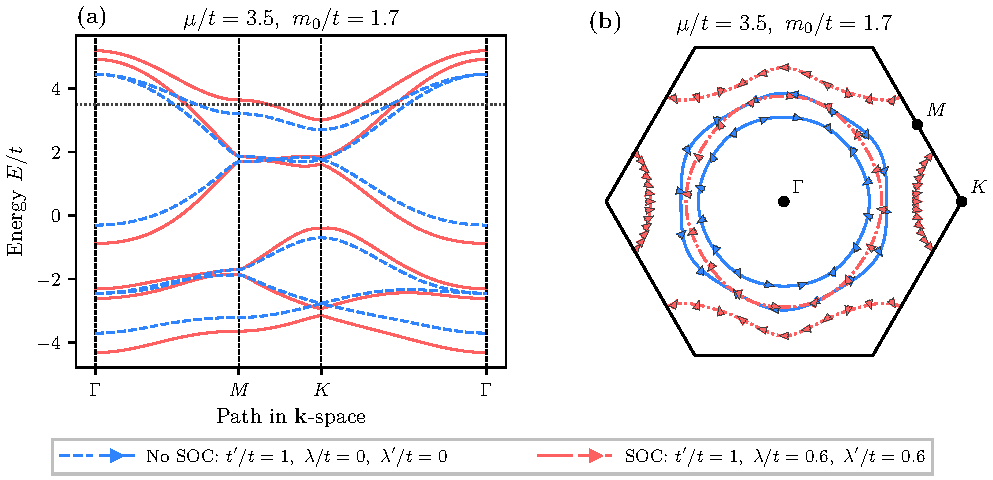
\includegraphics[
        width=\linewidth
    ]{Plots/Mn3Sn/Mn3Sn nonbreathing.pdf}
    \par\bigskip
    \begin{subfigure}[t]{0.46\textwidth}
        \centering
        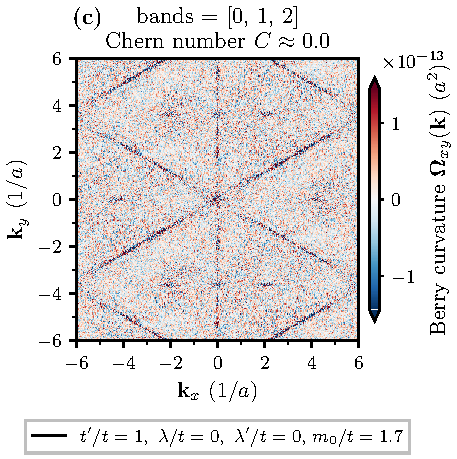
\includegraphics[
            width=\linewidth
        ]{Plots/Mn3Sn/Mn3Sn nonbreathing_berry_wo_soc.pdf}
        
    \end{subfigure}
    \hfill
    \begin{subfigure}[t]{0.48\textwidth}
        \centering
        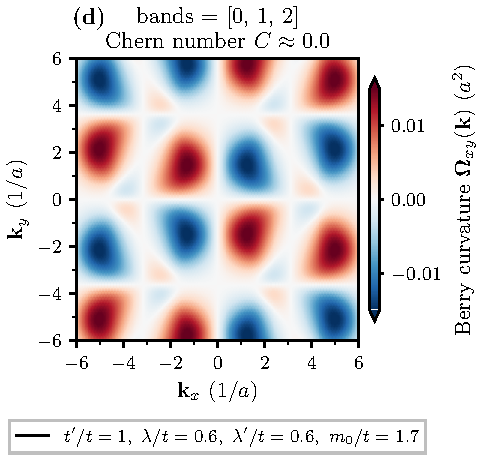
\includegraphics[
            width=\linewidth
        ]{Plots/Mn3Sn/Mn3Sn nonbreathing_berry_w_soc.pdf}
        
    \end{subfigure}
    \caption{\textbf{Tight-binding results for \ce{Mn3Sn} in the nonbreathing limit, with the magnetic texture shown in Fig.~\ref{fig: magnetic texture Mn3Ge and Sn}~(b), obtained using the Bloch Hamiltonian in Eq.~\eqref{eq: bloch-Hamiltonian}.} (a) Electronic band structure along the high-symmetry path $\Gamma$--$M$--$K$. (b) In-plane spin texture on the Fermi surface at the chemical potential $\mu$. (c,d) Berry curvature calculated without and with spin--orbit coupling (SOC), respectively, using the Fukui--Hatsugai--Suzuki method described in Eq.~\eqref{eq: berry curv comp}.}
    \label{fig:Mn3Sn-nonbreathing}
\end{figure}
In the nonbreathing limit, in the presence of SOC, we are able to observe the constraints given by the $\mathcal{M}$ plane, which force the spins to align perpendicular to it  on the mirror-invariant momentum line and the Berry curvature to vanish on it. A mirror-symmetric Fermi-surface spin texture can be seen in Fig.~\ref{fig:Mn3Sn-nonbreathing} (b).
In the nonbreathing limit, we expect the $[E||C_{2z}]$-symmetry, imposing evenness in the electronic-structure energy, spins and Berry curvature. \\
Note that none of the constraints imposed by the symmetry $[C_{3z}||C^{-1}_{3z}]$ according to Eq.~\eqref{eq: C_3z^-1 symm} can be observed in the presence of SOC, which is consistent with the found $[C_{3z}||C_{3z}^{-1}]$ symmetry breaking in the presence of SOC. 
\begin{figure}[htbp]
    \centering
    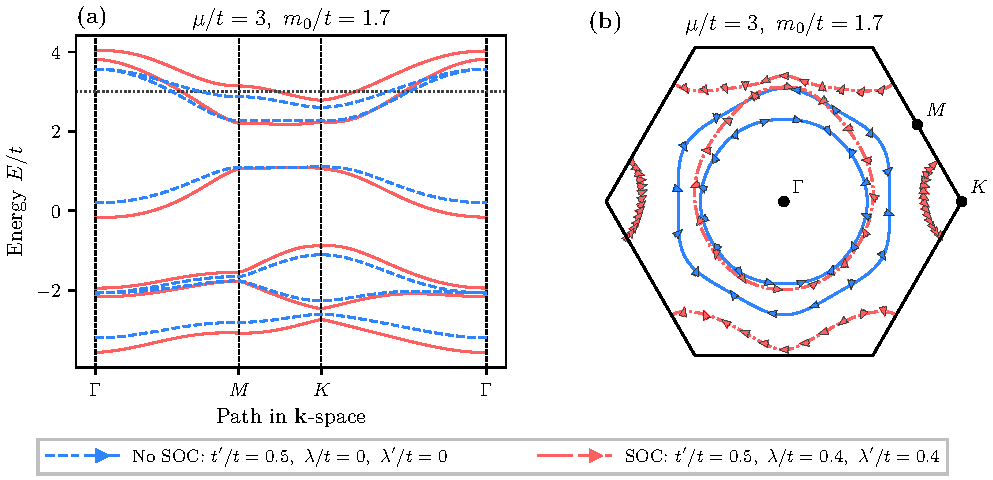
\includegraphics[
        width=\linewidth
    ]{Plots/Mn3Sn/Mn3Sn breathing.pdf}
    \par\bigskip
    \begin{subfigure}[t]{0.48\textwidth}
        \centering
        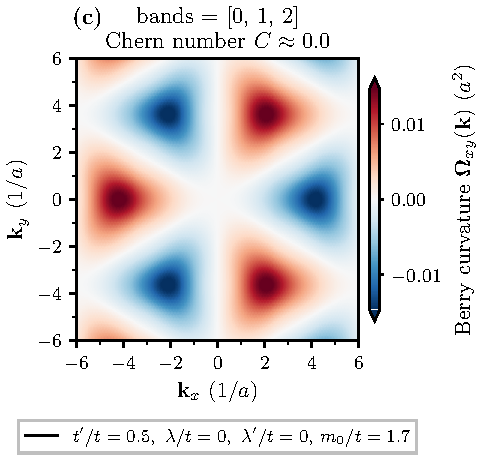
\includegraphics[
            width=\linewidth
        ]{Plots/Mn3Sn/Mn3Sn breathing_berry_wo_soc.pdf}
        
    \end{subfigure}
    \hfill
    \begin{subfigure}[t]{0.48\textwidth}
        \centering
        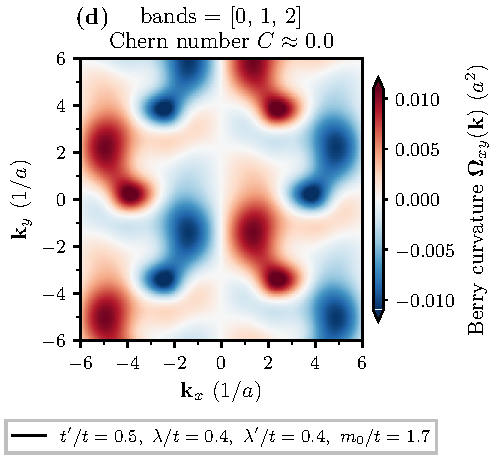
\includegraphics[
            width=\linewidth
        ]{Plots/Mn3Sn/Mn3Sn breathing_berry_w_soc.pdf}
        
    \end{subfigure}
    \caption{\textbf{Tight-binding results for \ce{Mn3Sn} in the breathing lattice, with the magnetic texture shown in Fig.~\ref{fig: magnetic texture Mn3Ge and Sn}~(b), obtained using the Bloch Hamiltonian in Eq.~\eqref{eq: bloch-Hamiltonian}.} (a) Electronic band structure along the high-symmetry path $\Gamma$--$M$--$K$. (b) In-plane spin texture on the Fermi surface at the chemical potential $\mu$. (c,d) Berry curvature calculated without and with spin--orbit coupling (SOC), respectively, using the Fukui--Hatsugai--Suzuki method described in Eq.~\eqref{eq: berry curv comp}.}
    \label{fig:Mn3Sn-breathing}
\end{figure}
Switching to a breathing kagome lattice, the symmetry $[E||C_{2z}]$ is broken, so no longer enforcing evenness. The mirror plane $\mathcal{M}$ perpendicular to the $x$-axis is evident from the vanishing Berry curvature in Fig.~\ref{fig:Mn3Sn-breathing} (d) and in the in-plane Fermi-surface spin texture in Fig.~\ref{fig:Mn3Sn-breathing} (b). The property in Eq.~\eqref{eq: symmetry_M} can also be confirmed by rotating the spins around the $x$-axis and mapping them to the reflected momentum. The only observable symmetry is $\mathcal{M}$ in the presence of SOC and breathing, which is preserved by the system.\\

The mirror plane forces the net magnetization to vanish along  the $y$- and $z$-directions. Analogously to \ce{Mn3Ge}, the broken $[C_{3z}||C_{3z}^{-1}]$ symmetry in the presence of SOC allows an in-plane net magnetization. Thus, an $x$-directed net magnetization is allowed. 

The magnetic order is fully compensated because the three equal-magnitude moments separated by $120^\circ$ sum to zero, as depicted in Fig.~\ref{fig: magnetic texture Mn3Ge and Sn}~(b). 
\ce{Mn3Sn} exhibits spin-split bands also in the absence of SOC. Thus, with full compensation and the spin-split bands, \ce{Mn3Sn} is classified as a strong altermagnet. 
Hence, \ce{Mn3Sn} is a strong altermagnet of M-type, like \ce{Mn3Ge}, exhibiting an $x$-directed net magnetization in the presence of SOC. Therefore, our result agrees with the classification given in Ref.~\cite{Cheong2025}.\\
The effects of the net magnetization can also be seen in the in-plane Fermi-surface spin textures for $k_x=0$, shown in Figs.~\ref{fig:Mn3Sn-nonbreathing} and \ref{fig:Mn3Sn-breathing}, in the presence of SOC. 
Analogously to \ce{Mn3Ge}, we show the effect of magnetization on the Fermi surface.
In the presence of SOC, the Fermi-surface spin textures in Figs.~\ref{fig:Mn3Sn-nonbreathing} and \ref{fig:Mn3Sn-breathing} exhibit a deformation along $k_y$. The mirror symmetry constrains the spins on the mirror plane $k_x=0$ to point along the $x$-direction. Therefore, the energy shift of the Rashba term, obtained by taking its expectation value, is $\Delta E_n=-\alpha_{\mathrm R}k_y\langle\sigma_x\rangle_n$, leading to an increase or decrease of the spin-split energy, depending on the sign of the spin expectation value. This deformation of the Fermi surface is observed.
 
Thus, the net magnetization supports the classification of \ce{Mn3Sn} as an M-type altermagnet, as defined in Ref.~\cite{Cheong2025}.